\chapter{Opis projektnog zadatka}

    \section{Motivacija}
    Cilj je razviti mobilnu aplikaciju koja će pomoći pri obavljanju kupovine u
    dućanima. Prije odlaska u trgovinu ljudi često pišu popis namirnica koje trebaju
    kupiti. Pritom im je nerijetko bitan ukupan iznos kupovine, a posebno
    ima li željenog proizvoda u trgovini u koju namjeravaju ići. Aplikacija
    „SmartCart” će omogućiti kupcima da sastave
    popis namirnica za kupovinu i izračunati njihovu cijenu na temelju
    podataka o cijenama koje u aplikaciju mogu unijeti trgovci. Popis će imati
    mogućnost pretvaranja u košaricu tijekom kupnje kad se namirnice
    uzimaju s polica, tj. praćenja cijene uzetih namirnica, za one koji se
    ne drže popisa u potpunosti. To će također ubrzati proces kupovine namirnica pa će ljudi manje vremena provoditi u trgovini i bit će manje gužve. Osim toga, trgovcima će to biti odlična promocija jer će oni kupci kojima je svejedno u koju trgovinu idu, moći vidjeti onu s najmanjom cijenom namirnica u blizini. 
    
    \section{Opis rada sustava}
    Budući da je srž aplikacije mogućnost stvaranja popisa, prikaz popisa se otvara i prilikom pokretanja aplikacije. Na popise se mogu dodavati artikli na četiri načina:
    \begin{packed_item}
        \item Skeniranjem barkoda artikla - dodaje se točno određeni artikl zadan barkodom i na popis i u košaricu
        \item Pretragom i odabirom - dodaje se određeni artikl na popis pretragom imena (koja dopušta manje pogreške prilikom unosa)
        \item Zadavanjem filtra - na popisu se nalazi onaj artikl koji najbolje zadovoljava filtar i redukcijsku funkciju (npr. najmanja cijena) u trenutku zadnjeg osvježavanja. Količina dostupnih filtra i redukcijskih funkcija će se mijenjati tijekom razvoja aplikacije. Primjeri funkcija filtra su "Cijena unutar intervala", "Vrsta proizvoda" i "Proizvedeno u", a primjeri redukcijskih funkcija su "Najmanja cijena" i "Najveća cijena po kilogramu"
        \item Dodavanjem iz popisa omiljenih artikala
    \end{packed_item}
    
    Dodanim proizvodima moguće je mijenjati količinu, pregledati informacije ili ih dodati u popis omiljenih artikala, na popisu označenih zvjezdicom, koji se nalazi u bočnoj traci. Svaki se popis sastoji od artikala, njihovih količina i cijena (svaka cijena je povezana s nekom trgovinom). Artikle možemo dodati više puta na isti popis. Korisnik artikle na popisu može označiti dodanima u košaricu. Ukupna cijena košarice, kao i cijena cijelog popisa su prikazane uz popis. Moguće je imati više popisa. Moguća je potpuna manipulacija popisima – stvaranje, brisanje, kopiranje, zatvaranje i otvaranje. Popisi su pohranjeni lokalno na korisničkom uređaju. \\
    
    Budući da svaki trgovac zadaje svoju cijenu za artikle na popisu, postoje tri načina izračuna cijena:
    \begin{packed_item}
        \item Najjeftinija trgovina - korisnik prepušta sustavu da nađe najbližu trgovinu za koju je zbroj cijena svih artikala na popisu najmanji.
        \item Najjeftiniji artikli - korisnik prepušta sustavu da za svaki artikl nađe najbližu trgovinu u kojoj je cijena tog artikla najmanja
        \item Određena trgovina - korisnik pretražuje trgovine i odabire jednu te se cijene osvježe u skladu s time. Ovo je pretpostavljeni način
    \end{packed_item}
    
    Budući da se informacije o trgovinama i cijenama u njima često mijenjaju, korisnik može osvježavati svoje popise. Pritom bojanje oznake količine proizvoda crveno označava da proizvod nije više dostupan u trgovini s kojom je povezan na popisu. Bojanje imena proizvoda crveno označava da proizvod nije više dostupan niti u jednoj trgovini, a bojanje cijene proizvoda crveno ili zeleno označava da se ta cijena redom povećala ili smanjila. \\
    
    Informacije o trgovini moguće je pronaći pritiskom na cijenu artikla u toj trgovini. Tu je moguće pronaći radno vrijeme, adresu, poveznicu za prikaz trgovine na \textit{Google Maps} karti te udaljenost od trgovine ako je dozvoljen pristup lokaciji. \\
    
    Informacije o artiklima i dostupnosti u trgovinama ne spremaju se na uređaju, pa je internetska veza s poslužiteljem nužna za cjelovitu funkcionalnost aplikacije. Aplikacija je u "online" načinu rada ako je povezana s poslužiteljem. Prekidom "online" načina rada aplikacija prelazi u "offline" način rada. Bez veze s poslužiteljem korisnik samo može micati artikle s popisa te stvarati, brisati, otvarati i zatvarati popise bez dodavanja novih artikala. Jedino što je spremljeno u bazi podataka na uređaju su podatci o artiklima na popisima te među omiljenim artiklima. \\
    
    Sva ova funkcionalnost dostupna je neprijavljenom korisniku, tj. \underbar{gostu}. No, potrebno je i nabaviti informacije koje bi se prikazivale u aplikaciji. Neki će pisati korisne infromacije, ali kako bi se zaustavilo one koji bi širili dezinformacije, za upis bilo kakvih informacija potrebno je imati korisnički račun koji administrator prema potrebi može onemogućiti. Neprijavljeni korisnici ne mogu promijeniti informacije o artiklu ni samo na uređaju, kako bi se potaknulo korisnike da podijele podatke koje steknu. \\
    
    Dakle, postoji tri vrste korisnika s korisničkim računom:
    \begin{packed_item}
        \item Kupac
        \item Trgovac
        \item Administrator
    \end{packed_item}
    
    \underbar{Kupac} može, uz osnovnu funkcionalnost koju ima i gost, mijenjati informacije o artiklu, ali samo one koje nisu nužno vezane uz trgovinu. Dakle, opis artikla u pravilu nije vezan uz trgovinu. Samo cijena, popust i dostupnost. Kupac o svim informacijama o artiklu i/ili trgovini može glasati, a na temelju toga se izračunava ocjena pouzdanosti koju vide svi korisnici uz opis. Također, kako bi se povećala vjerojatnost da onaj tko piše informacije o artiklu piše točne podatke, prije spremanja izmijenjenih podataka mora očitati barkod artikla. Za registraciju su mu potrebni samo email i lozinka. \\
    
    \underbar{Trgovac}, uz funkcionalnost kupca, ima i mogućnost dodavanja svojih trgovina te manipulacije njima. Za stvaranje trgovine su mu potrebni lokacija trgovine i radno vrijeme. Trgovac kroz svoju nadzornu ploču na kojoj ima pregled trgovina koje je dodao i proizvoda u njima dodaje ili mijenja artikle kao petorku (barkod, cijena, popust, dostupnost, email adresa željenog opisivača). Barkod je potreban da bi korisnici znali da je taj proizvod u toj trgovini, cijena i popust određuju ukupnu cijenu proizvoda koja će pisati na popis, a dostupnost označava ima li artikla u trgovini bez da ga se briše. Trgovac ne mora unositi opis artikla, ali ako postavi email adresu željenog opisivača i korisnik s tom email adresom je napisao opis o artiklu s tim barkodom, taj opis nadjača ostale kad se prikazuje cijena artikla u toj trgovini. Inače se informacije o artiklu u trgovini povezuju s najpouzdanijim opisom. Nove informacije o artiklima se mogu učitati i iz csv datoteke jednakog rasporeda stupaca. Kako bi se smanjila vjerojatnost lažnog predstavljanja i neispravnih informacija o cijenama i dostupnosti artikala u trgovini, trgovac za registraciju mora upisati tajni broj koji je dobio (uživo) od administratora i samo on smije mijenjati informacije o trgovinama. Tu je ipak novac "u igri". \\
    
    \underbar{Administrator} ima zadaću održavati red u sustavu. Može vidjeti sve podatke (poput broja glasova na opisima trgovaca i kupaca te njihovih mail adresa, lozinke su sakrivene SHA-256 algoritmom), a mijenjati može informacije o artiklima, kao i kupac. Može onemogućiti pristup bilo kojem korisničkom računu, uključujući trgovce i druge administratore (za micanje privilegija administratoru ipak treba najmanje pola glasova administratora u istom danu). Trgovcu, iako ne može mijenjati informacije o trgovini, može ukloniti trgovinu kako bi se ipak spriječilo zlonamjerno iskorištavanje sustava. Administrator također privilegije stiče registracijom uz tajni broj koji dobije (uživo) od drugih administratora. \\
    
    \section{Mogućnosti proširenja}
    
    Iako je aplikacija u ovom obliku potpuno funkcionalna, ako preraste u pravi proizvod postoji više mogućnosti proširenja i poboljšanja korisničkog iskustva:
    \begin{packed_item}
        \item Proširenje mogućnosti korištenja u načinu rada bez veze s poslužiteljem
        \item Slike artikala
        \item API za trgovce i/ili kupce
        \item Spremanje popisa u bazu na poslužitelju
        \item Dijeljenje popisa
        \item Praćenje cijene artikala kroz vrijeme
        \item Tlocrt trgovina i promjena poretka artikala na popisu
        \item Podržavanje popusta vezanih uz kartice vjernosti
        \item Posredovanje u "online" kupovini
        \item Suradnja sa stranicom poput Coolinarike za ubacivanje sastojaka jela na korisnički popis
        \item Definiranje maksimalnog broja trgovina po kojima se podijele sastojci iz košarice za izračun minimalne cijene (trenutno postoje dvije krajnosti: 1 i broj artikala)
    \end{packed_item}
    
    
    \section{Slične aplikacije}
    
    U nastavku su navedene dvije aplikacije čija je funkcionalnost slična onoj naše aplikacije. Ipak, valja naglasiti da nam one nisu ni inspiracija niti ih nastojimo imitirati. One su upravo to - aplikacije s nekim funkcionalnostima sličnima našoj.
    
    \subsection{SmartCart: Shopping list}
    
    Ova aplikacija (\ref{fig:SmartCart: Shopping list}) je slična našoj po tome što ima funkcionalnost stvaranja više popisa i manipulacije njima. Bitna razlika je to što nema "agregator cijena" nego sve cijene upisuje korisnik. Za ovu aplikaciju smo saznali tek nakon definiranja specifikacije programske potpore, nakon pretrage trgovine \textit{Google Play} za potrebe ove dokumentacije, zato ima vrlo slično ime i neke detalje jer izgleda da slično razmišljamo.
    
    \begin{figure}
        \centering
        \begin{subfigure}{0.49\textwidth}
            \centering
            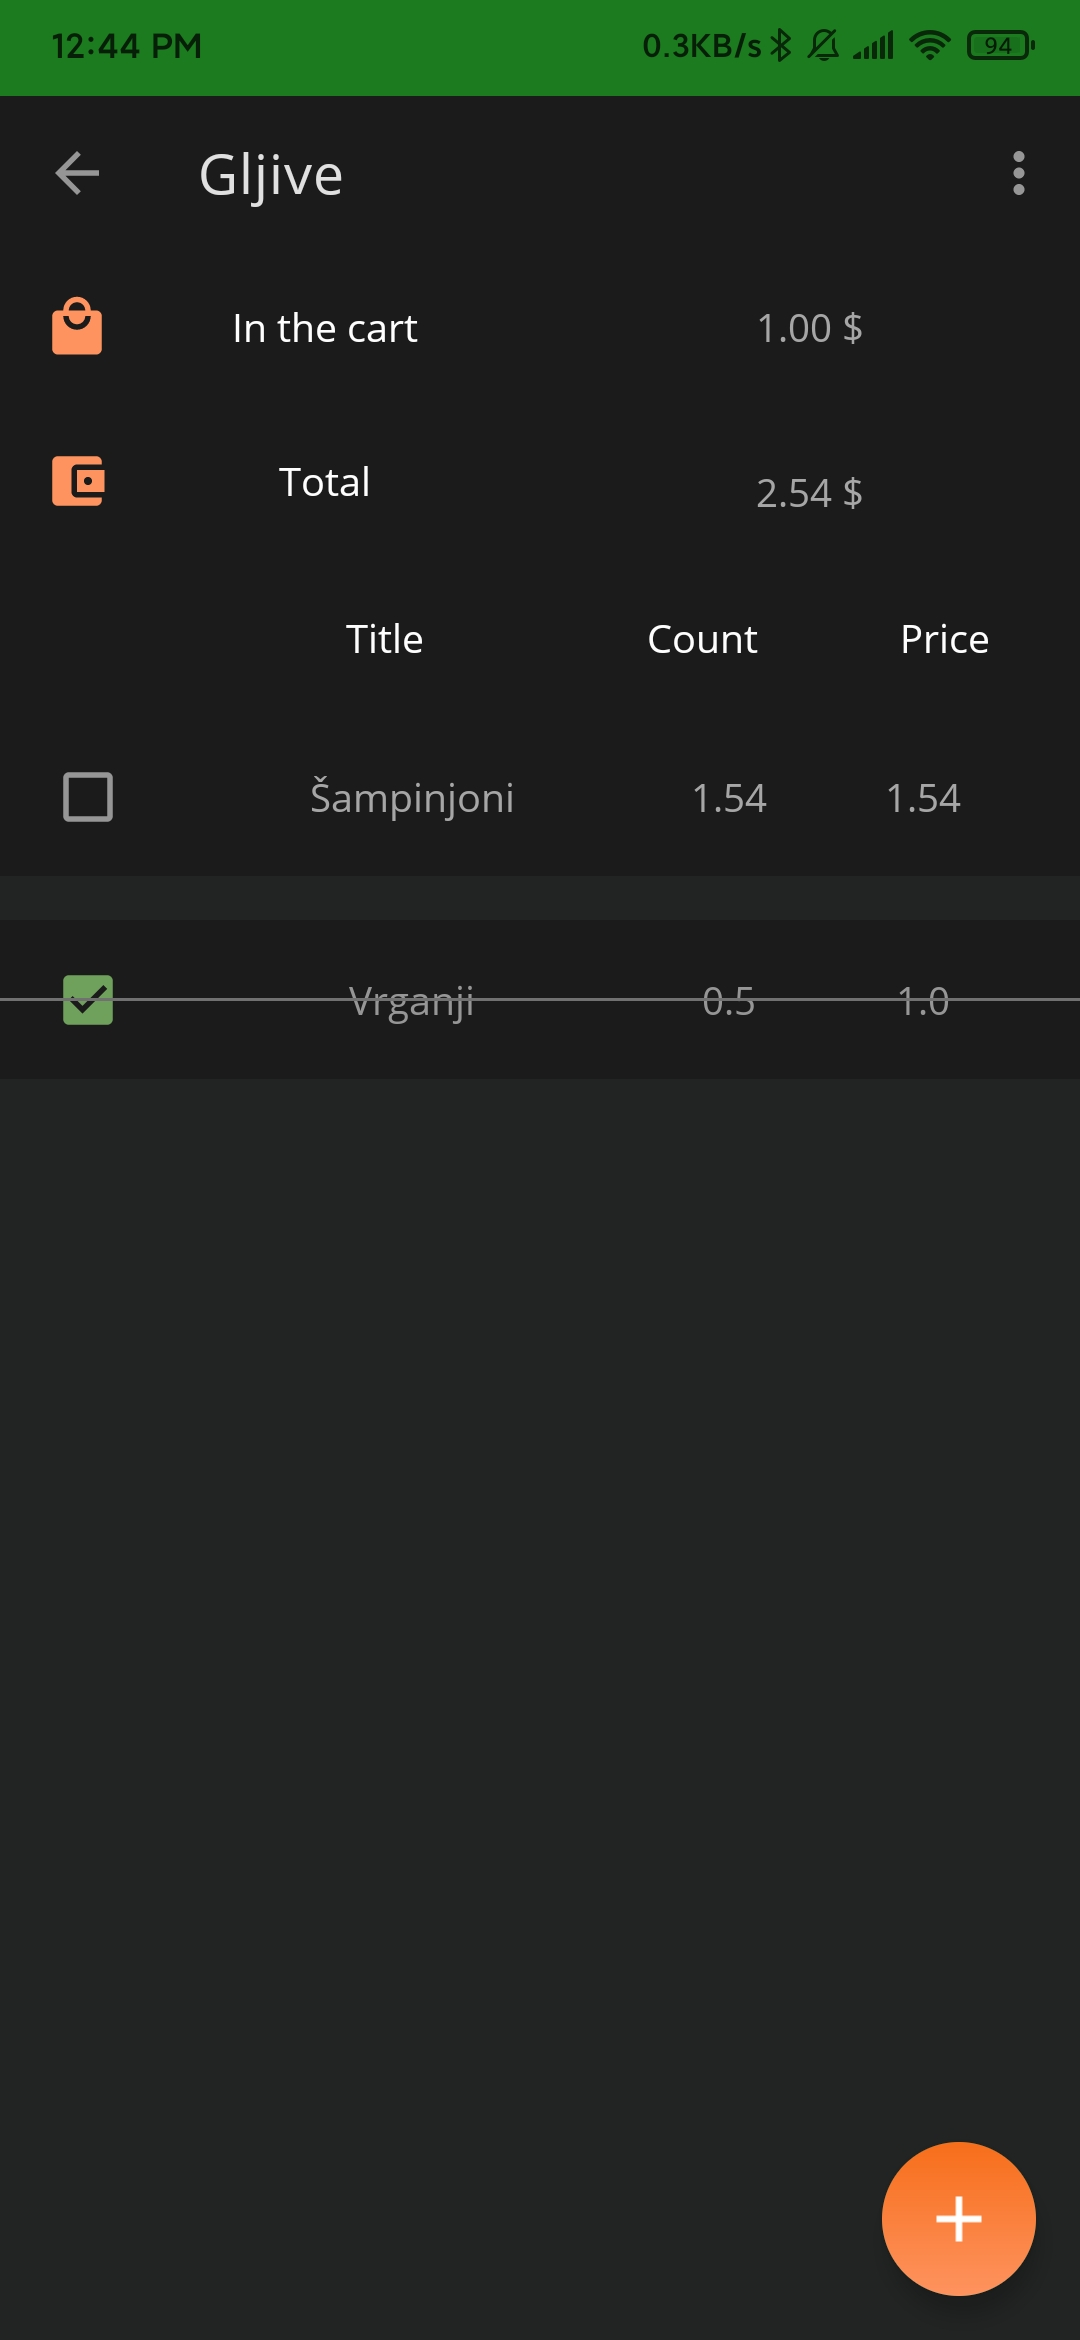
\includegraphics[width = \textwidth]{slike/Informerlab.jpg}
            \caption{SmartCart:Shopping list}
            \label{fig:SmartCart: Shopping list}
        \end{subfigure}
        \begin{subfigure}{0.49\textwidth}
            \centering
            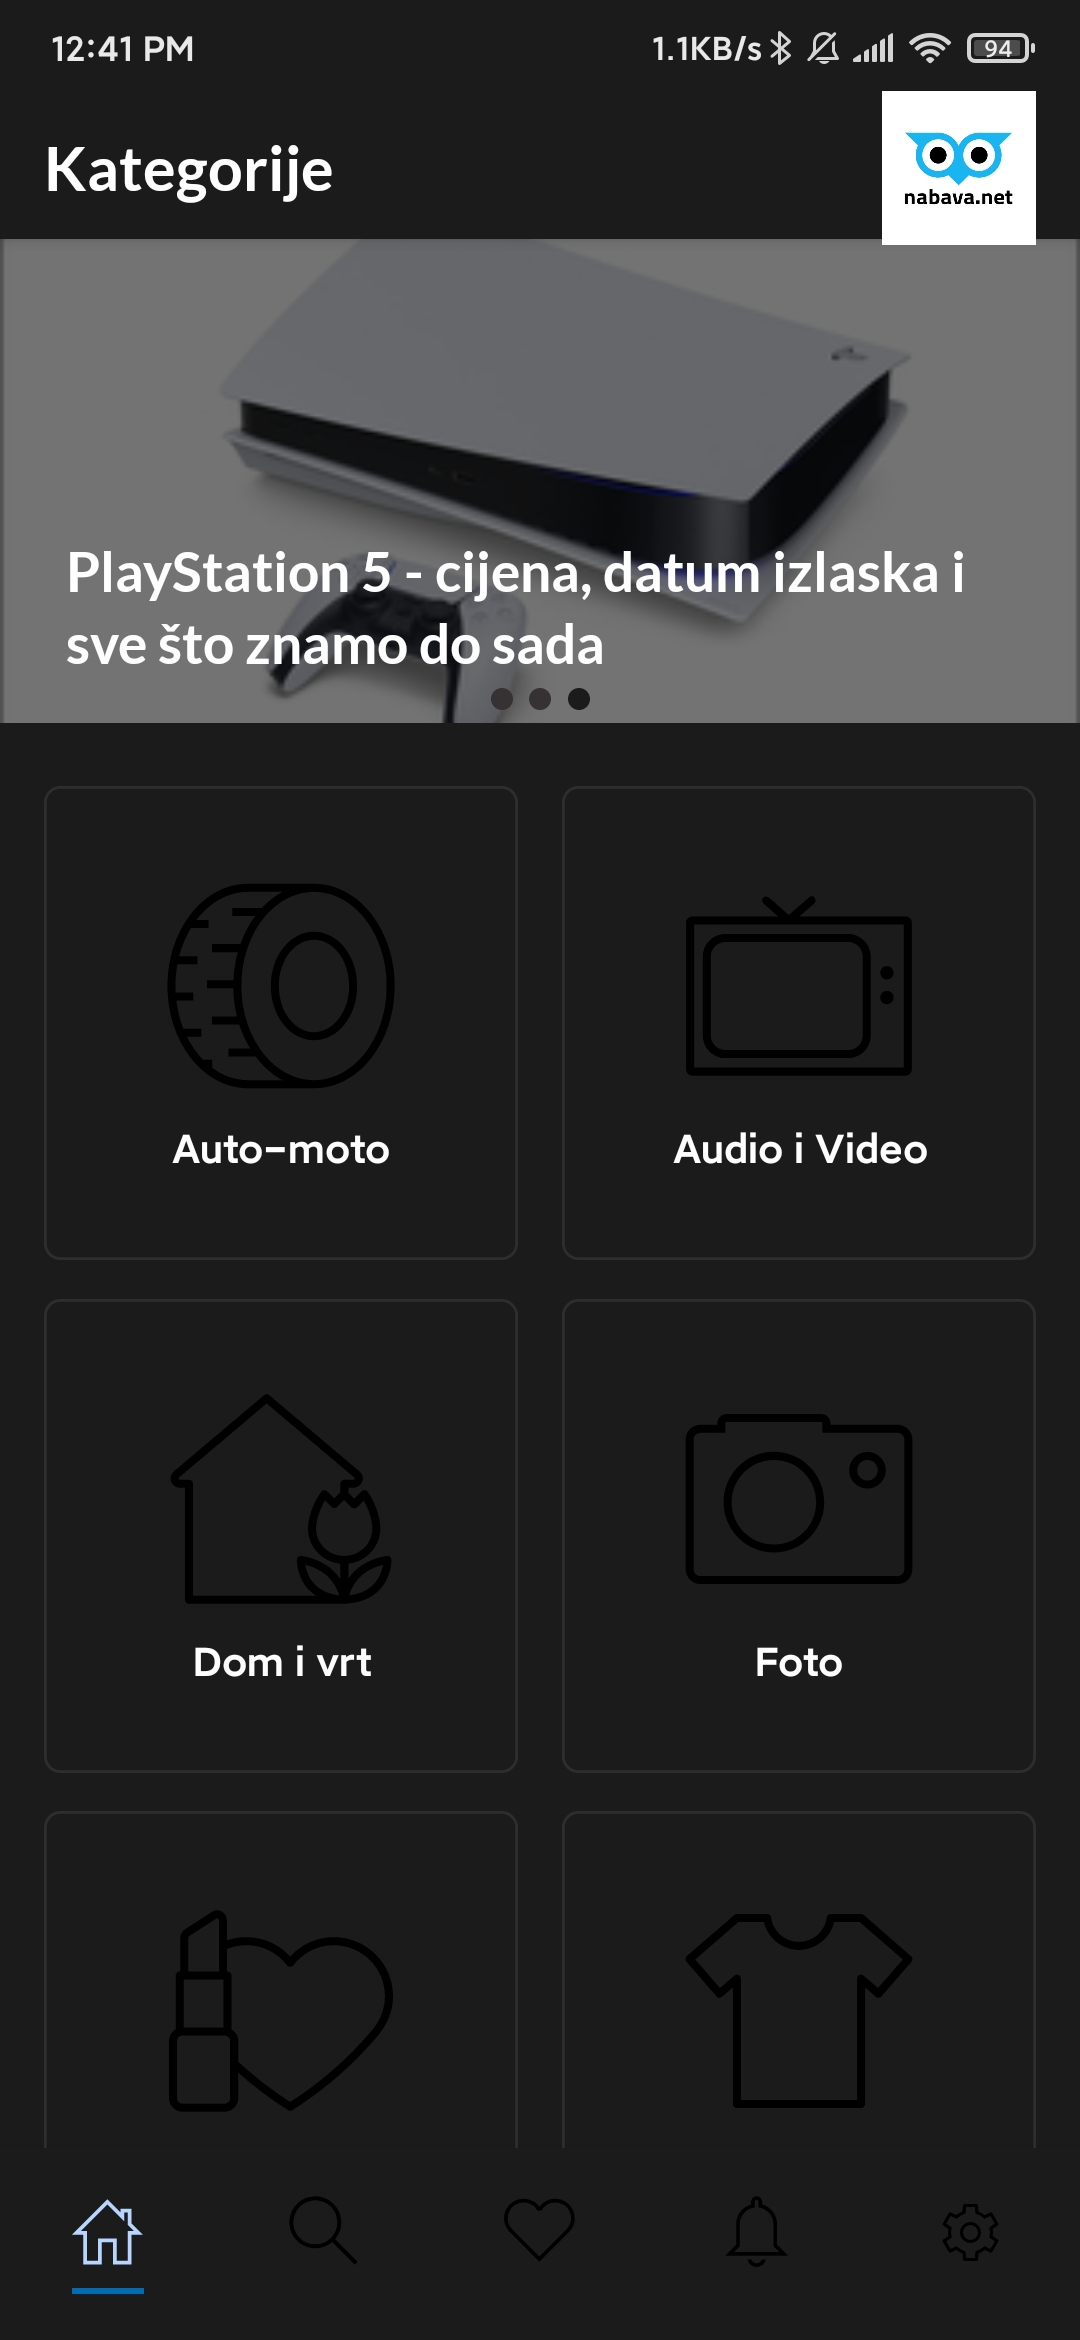
\includegraphics[width = \textwidth]{slike/nabava_net.jpg}
            \caption{nabava.net}
            \label{fig:nabava.net}
        \end{subfigure}
        % \label{fig:combined}
    \end{figure}
    
    
    \subsection{nabava.net}
    
    Aplikacija nabava.net (\ref{fig:nabava.net}) ima upravo suprotno - "agregator cijena", ali nema košaricu i usredotočena je na "online" kupovinu. Nije toliko usredotočena na namirnice. Mobilna aplikacija joj je zapravo prilagodba web aplikacije.
    
        
        \eject
        
    
